\chapter{气体的性质}\label{chapter-properties-of-gases}


\section{气体的状态和状态参量}
我们研究物理学问题时,经常要用一些物理量来描述研
究对象.问题不同,所用的物理量也不同.在力学中我们用位置、速度等物理量来描述物体的运动状态.
现在研究气体的热学性质,我们要用体积、压强、温度等物理量来描述气体的状态.描述气体状态的这几个物理量叫做气体的\NoteBold{状态参量}.

气体分子可以自由移动,因而气体总要充满整个容器.
气体的体积就是指气体所充满的容器的容积.
在国际单位制中,体积的单位有$ \UmcA $、$\UdmcA$、$ \UcmcA$等.日常生活和生产中还常用升作单位,升的国际代号是$\ULA$.
\[1 \UL =10^{-3} \Umc =1 \Udmc\]

气体对器壁有压力的作用,这是气体分子频繁地碰撞器壁而产生的.用打气筒把空气打到自行车的车胎里去,会把车胎胀得很硬,就是因为空气对车胎有压力而造成的.气体作用在器壁单位面积上的压力叫做气体的压强.

在国际单位制中,压强的单位是\NoteBold{帕斯卡},简称帕,国际代号是$\UPaA$.
$1 \UPa=1 \UNmq$.气体的压强还常用标准大气压($\UatmA$)和毫米汞柱($\UmmHgA$)作单位.
\[1 \Uatm =760 \UmmHg=1.013\times 10^5 \UPa \]
\[1 \UmmHg =133.3 \UPa \]

\begin{figure}[htbp]
    \centering
    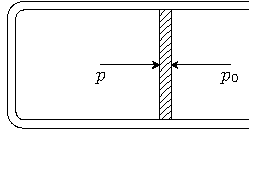
\includegraphics{fig/B/3-1.pdf}
    \caption{气体的压强等于大气压}\label{fig_B_3-1}
\end{figure}



在图~\ref{fig_B_3-1} 中,容器内的气体被活塞封闭着,当活塞静止不动时,容器内的气体对活塞的压力跟大气压对活塞的压力平
衡,所以这时容器内的气体的压强$p$等于大气压$p_0$,即$p=p_0$.如图~\ref{fig_B_3-2} 所示,用长为$h$的一小段水银柱把气体封闭在玻
璃管里.玻璃管水平放置时,被封闭的气体的压强$p_1$等于
大气压$p_0$,即$p_1=p_0$.玻璃管开口向上竖直放置时,气体的压强$p_2$等于大气压$p_0$加上这小段水银柱产生的压强$p_h$,即$p_2=p_0+p_h$.玻璃管开口向下竖直放置时,气体的压强$p_3$加上这小段水银柱产生的压强$p_h$等于大气压$p_0$,即$p_3+p_h=p_0$,由此得到$p_3=p_0-p_h$.

\begin{figure}[htbp]
    \centering
    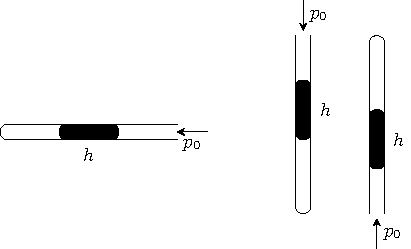
\includegraphics{fig/B/3-2.pdf}
    \caption{}\label{fig_B_3-2}
\end{figure}

温度这个物理量大家都很熟悉.温度是表示物体冷热程度的物理量,是物体分子热运动的平均动能的标志.温度的数值表示法叫做温标.
我们在初中学过摄氏温标.
用摄氏温标表示的温度叫做摄氏温度.
在国际单位制中采用热力学温标(又常叫绝对温标).
这种温标将在第\ref{sec-B-3-4-thermodynamic-temperature-scale}节中讨论.

研究气体的性质,首先引起我们注意的是描述气体状态的这三个物理量的变化.举例来说,地面附近的空气变热以后向空中上升时,它的体积、压强和温度都发生变化.把氧气装入钢筒时,或者用户(工厂、医院)把氧气从钢筒中放出来使用时,氧气的体积、压强和温度都发生变化.内燃机气缸里的燃料混合物爆发时,这三个物理量也都发生变化.对一定质量的气体来说,如果体积、压强和温度这三个量都不改变,我们就说气体处于一定的状态中.
如果这三个物理量同时发生变化或者其中有两个发生变化,我们就说气体的状态改变了.对一定质量的气体来说,只有一个量改变而其他两个都不改变的情况,是不会发生的.那么,在气体的状态改变时,这三个物理量的变化是任意的,还是相互关联,遵循一定的规律?如果遵循一定的规律,这个规律又是什么?这就是本章讨论的中心课题.

下面,我们用实验方法先研究一定质量的气体在分别保持温度、体积不变时,其他两个量的变化规律,然后在此基础上确定三个状态参量的变化规律.


\subsection*{练习一}
\begin{enumerate}
    \item 什么叫气体的压强?举出气体对器壁有压力作用的几个实例.
    \item 大气压为750毫米汞柱时,等于多少帕?
        \item 在图~\ref{fig_B_3-2} 中,水银柱的长度为19厘米,大气压为
    760毫米汞柱.
    玻璃管开口向上竖直放置时,被封闭的气体的压强等于多少毫米汞柱?开口向下竖直放置时,等于多少毫米汞柱?
\begin{figure}[htbp]
    \centering
    \begin{subfigure}{0.4\linewidth}
        \centering
        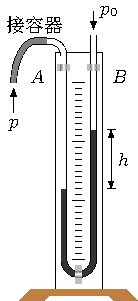
\includegraphics{fig/B/3-3a.pdf}
        \caption{}\label{fig_B_3-3a}
    \end{subfigure}
    \hfil
    \begin{subfigure}{0.4\linewidth}
        \centering
        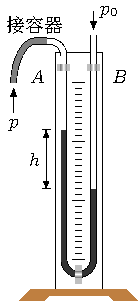
\includegraphics{fig/B/3-3b.pdf}
        \caption{}\label{fig_B_3-3b}
    \end{subfigure}
    \caption{}\label{fig_B_3-3}
\end{figure}


    \item 图~\ref{fig_B_3-3} 是测量气体压强的水银压强计,两端开口的U形管内装入水银,$A$管跟容器连接.已知大气压$p_0$和两管中水银面的高度差,就可以知道容器中气体的压强.大气压为$1.013\times 10^5 \UPa$,图~\ref{fig_B_3-3a} 和图~\ref{fig_B_3-3b} 中的$h$都是10厘米,分别求出这两种情形中气体的压强是多少帕.
    \item 在图~\ref{fig_B_3-4} 所示的几种情形中,被封闭的气体$A$的压强分别是多少帕?大气压为$1.013\times 10^5 \UPa $.
    \item 举出气体状态发生改变的几个实例.
\begin{figure}[htbp]
    \centering
    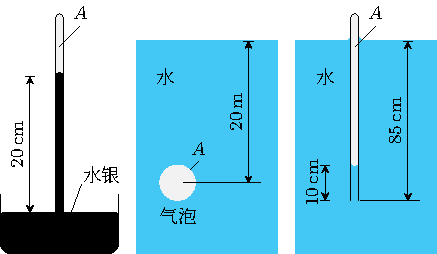
\includegraphics{fig/B/3-4.pdf}
    \caption{}\label{fig_B_3-4}
\end{figure}

\end{enumerate}

\section{气体的等温变化~~玻意耳--马略特定律}
我们先来研究温度不变时,一定质量的气体的压强随着
它的体积而变化的情形.这种变化叫做\NoteBold{等温变化}.
\begin{figure}[htbp]
    \centering
    \begin{subfigure}{0.3\linewidth}
        \centering
        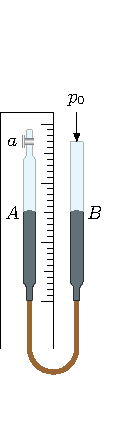
\includegraphics{fig/B/3-5a.pdf}
        \caption{}\label{fig_B_3-5a}
    \end{subfigure}
    \hfil
    \begin{subfigure}{0.3\linewidth}
        \centering
        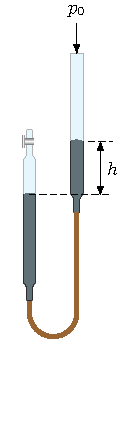
\includegraphics{fig/B/3-5b.pdf}
        \caption{}\label{fig_B_3-5b}
    \end{subfigure}
    \hfil
    \begin{subfigure}{0.3\linewidth}
        \centering
        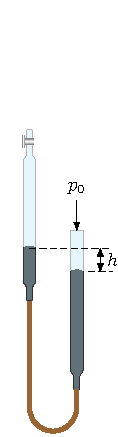
\includegraphics{fig/B/3-5c.pdf}
        \caption{}\label{fig_B_3-5c}
    \end{subfigure}
    \caption{}\label{fig_B_3-5}
\end{figure}

实验装置如图~\ref{fig_B_3-5} 所示,玻璃管$A$和$B$通过一条橡皮管连在一起.
$A$管上端有一个阀门$a$,$B$管上端是开口的.$A$管固定在有刻度的竖直板上,$B$管可以上下移动.
实验开始时,打开阀门$a$,从$B$管注入水银,然后关闭阀门,把一定质量的空气封闭在$A$管里.当两管中的水银面一样高时(图~\ref{fig_B_3-5a}),$A$管里空气的压强等于作用在$B$管水银面上的大气压.

把$B$管慢慢提高,使$A$管里空气的体积缩小.这时$B$管里的水银面比$A$管里的高(图~\ref{fig_B_3-5b}),$A$管里气体的压强等于大
气压加上$B$管水银面高出$A$管水银面的那段水银柱的压强.实验表明,在温度不变的条件下,气体的体积缩小到原来的几分之一,它的压强就增大到原来的几倍.

把$B$管慢慢放低,使$A$管里气体的体积增大,这时$B$管里的水银面比$A$管里的低(图~\ref{fig_B_3-5c}),$A$管里气体的压强等于大气压减去$A$管水银面高出$B$管水银面的那段水银柱的压强.实验表明,在温度不变的条件下,气体的体积增大到原来的几倍,它的压强就减小为原来的几分之一.

改用其他气体做这个实验,得到的结果相同.

英国科学家玻意耳($1627 \sim 1691$)和法国科学家马略特($1620 \sim 1684$)各自独立地用实验研究了气体的压强和体积的关系,得到下面的结论:

\NoteBold{温度不变时,一定质量的气体的压强跟它的体积成反比}.这个结论叫做\NoteBold{玻意耳--马略特定律}.

玻意耳--马略特定律可以用公式来表示.
保持一定质量气体的温度不变,设体积为$V_1$时压强为$p_1$,体积为$V_2$时压强为$p_2$,那么
\[\frac{p_1}{p_2}=\frac{V_2}{V_1} \]
或
\[p_1V_1=p_2V_2 \]

由此式可以看出,玻意耳--马略特定律也可以叙述为:

\NoteBold{温度不变时,一定质量的气体的压强跟它的体积的乘积是不变的}.其数学表达式为
\[pV=\text{恒量}\]

气体的等温变化也可以用图线来表示.用直角坐标系的
横轴表示气体的体积$V$,用纵轴表示气体的压强$p$.设在一定温度下,一定质量的某种气体在$V_1=2$升时,$p_1=1$标准大气压,在图~\ref{fig_B_3-6} 中由$A$点表示.根据玻意耳--马略特定律可以
得出:$V_2=4$升时,$p_2=1/2$标准大气压,由$B$点表示;$V_3=1$升时,$p_3=2$标准大气压,由$C$点表示;$V_4=1/2$升时,$p_4=4$标准大气压,由$D$点表示.当然还可以使气体的体积等于其他许多不同的数值,并计算出相应的压强的数值,从而得到其他许多点.由这些点连成的平滑曲线,叫做气体的等温线.从等温线可以清楚地看出温度不变时气体的压强跟体积的关系.
\begin{figure}[htbp]
    \centering
    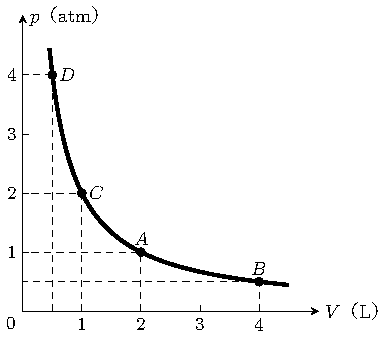
\includegraphics{fig/B/3-6.pdf}
    \caption{气体等温变化的图线}\label{fig_B_3-6}
\end{figure}

\begin{example}
某个容器的容积是10升,所装气体的压强是$20\times 10^5$帕.
如果温度保持不变,把容器的开关打开以后,容器
里剩下的气体是原来的百分之几?设大气压是$1.0\times 10^5$帕.
\end{example}

\begin{solution}
这个题目可以这样来分析.容器里装着一定质量的气体.
取这一定质量的气体作为我们的研究对象.气体在初状态时,$p_1=20\times 10^5$帕,$V_1=10$升.
打开开关以后,由于气体压强大于外界大气压,于是气体发生膨胀(等温膨胀),有一部分
气体跑出容器.
随着气体的膨胀,气体的压强降低.
最后,当气体压强等于外界大气压时,气体停止膨胀而达到末状态.这时,气体一部分在容器内,一部分在容器外.如果我们知道气体在末状态时占有多大体积,就可以知道容器里剩下的气体为原来的百分之几.

气体在初状态时,$p_1=20\times 10^5$帕,$V_1=10$升,在末状态时,$p_2=1.0\times 10^5$帕,$V_2$为待求的体积.由玻意耳--马略特定律$p_1V_1=p_2V_2$得到
\[V_2=\frac{p_1V_1}{p_2}=\frac{20\times 10^5\times 10}{1.0\times 10^5} \UL =200\UL \]

这时容器里剩下10升气体,所以剩下的气体是原来气体的$10 \UL /200\UL=5\%$.
\end{solution}

从这里我们看到,利用玻意耳--马略特定律来解题,先要明确研究对象以及它的初末两个状态,然后才能利用公式来求解.
用玻意耳--马略特定律解题时,还要注意等式两边的$p$或$V$必须采用相同的单位,至于具体采用什么单位,可以根据解题方便来决定.

玻意耳--马略特定律表示一定温度下气体的压强跟体积的关系,因此我们可以预料这个定律的表达式
\[pV=\text{恒量} \]
中的恒量跟温度有关系.实验表明,温度不同,这个恒量也不同.
图~\ref{fig_B_3-7} 中画出了不同温度下的几条等温线,从此可以知道:一定质量的气体,保持它的体积不变,温度越高,压强越大;保持它的压强不变,温度越高,体积越大.
可见,表达式中的恒量随温度而增大.这样看来,要确定体积、压强、温度这
三个物理量的变化规律,我们还需要研究压强怎样随着温度而变化或者体积怎样随着温度而变化.
\begin{figure}[htbp]
    \centering
    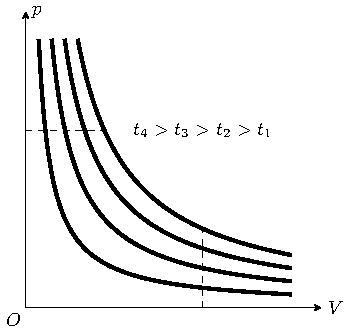
\includegraphics{fig/B/3-7.pdf}
    \caption{不同温度下的几条等温线}\label{fig_B_3-7}
\end{figure}



玻意耳--马略特定律是在压强不太大(和大气压比较)、温度不太低(和室温比较)的条件下总结出来的.在这种条件下,不论什么气体都近似地符合这个定律.当压强很大、温度很低时,由这个定律得出的结果跟实际测量的结果有很大差别,这个定律就不适用了.举例来说,有一定质量的氦气,压强为1标准大气压时,体积为$1\Umc$.压强为500标准大气压时,按照玻意耳--马略特定律体积应该是$1/500 \Umc $,而实际测量的结果是$1.36/500\Umc$,二者之间已经显示出不小的差别.压强为1000标准大气压时,按照玻意耳-马略特定律体积应该是$1/1000\Umc$,而实际测量的结果是$2.0685/1000\Umc$,二者相差一倍多,根本无法应用玻意耳--马略特定律了.


\subsection*{练习二}
\begin{enumerate}
    \item 把打气筒的出口堵住,往下压打气筒的活塞,会感到越往下压越费劲.
    怎样解释这个现象?
    \item 某个容器的容积是5升,里面所装气体的压强是10标准大气压.
    如果温度保持不变,把容器的开关打开以后,这些气体会有多大体积?容器里剩下的气体是原来的百分之几?设外界压强为1标准大气压.
    \item 在上题里,打开容器的开关以后,气体的密度怎样改变?设上题里容器里剩下的气体的密度是$\rho_2$,原来容器里气体的密度是$\rho_1$,那么,密度之比$\rho_2/\rho_1$是多大?
    \item 在密闭圆筒的中央有一个活塞(图~\ref{fig_B_3-8}),活塞两边
    封闭着两部分气体,它们的压强都是750毫米汞柱.
    现在用
    力把活塞向右移动,使活塞右边气体的体积为原来的一半,那么活塞两边气体的压强差是多大?假定气体的温度不变.
\begin{figure}[htbp]
    \centering
    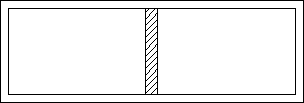
\includegraphics{fig/B/3-8.pdf}
    \caption{}\label{fig_B_3-8}
\end{figure}

    \item 在图~\ref{fig_B_3-2} 中,水银柱的长度为19厘米,大气压为760毫米汞柱.
    玻璃管是粗细均匀的.
    玻璃管开口向上竖直放置时,被封闭的气体柱长15厘米,当开口向下竖直放置时,被封闭的气体柱的长度是多少?
    \item 在下端封闭的竖直玻璃管里有一段4厘米长的水银柱,水银柱下面封闭着6$\Ucmc$的空气.
    玻璃管的横截面积是0.1$\Ucmq$.如果再向管里装入27.2克水银,那么,封闭在水银
 柱下面的空气柱有多高?设大气压为760毫米汞柱.
    \item 一个足球的容积是2.5升.用打气筒给这个足球打气,每打一次就把1标准大气压的空气打进去125$\Ucmc$.
    如果足球在打气前内部没有空气,打了40次以后,足球内部空气的压强有多大?假定空气的温度不变.
\end{enumerate}

\section{气体的等容变化~~查理定律}
气体在体积不变的情况下发生的变化叫做等体积变化,也叫\NoteBold{等容变化}.现在我们用实验来研究一定质量的气体,在体积保持不变的情况下它的压强怎样随着温度而变化.


实验装置如图~\ref{fig_B_3-9} 所示,烧瓶上连一根玻璃管,用橡皮管把它跟水银压强计连在一起,这样便在烧瓶中封入了一定质量的气体.调节压强计的可动管$A$,使两管中的水银面一样高,这时瓶里气体的压强就等于当时的大气压强(图~\ref{fig_B_3-9a}).
用记号标出$B$管中水银面的位置.


\begin{figure}[htbp]
	\centering
	\begin{subfigure}{0.3\linewidth}
		\centering
		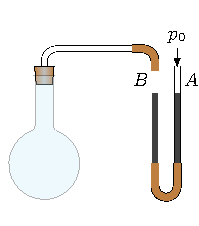
\includegraphics{fig/B/3-9a.pdf}
		\caption{}\label{fig_B_3-9a}
	\end{subfigure}
	\hfil
	\begin{subfigure}{0.3\linewidth}
		\centering
		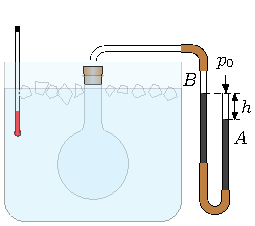
\includegraphics{fig/B/3-9b.pdf}
		\caption{}\label{fig_B_3-9b}
	\end{subfigure}
	\hfil
	\begin{subfigure}{0.3\linewidth}
		\centering
		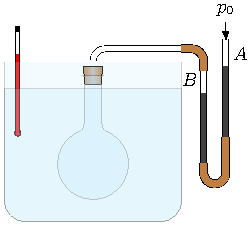
\includegraphics{fig/B/3-9c.pdf}
		\caption{}\label{fig_B_3-9c}
	\end{subfigure}
	\caption{}\label{fig_B_3-9}
\end{figure}


把烧瓶放进盛着冰水混合物的容器里,经过一段时间,瓶里气体的温度跟冰水混合物的温度一样,等于0$\Ucede$.调节压强计的$A$管,使$B$管中水银面恢复到原先标出记号的位置,也就是使气体恢复原来的体积.从压强计$B$管的水银面比$A$管的水银面高可以知道,气体压强减小了(图~\ref{fig_B_3-9b}).

把烧瓶放进盛有热水的容器中,调节压强计的$A$管,使$B$管中水银面恢复到原先标出记号的位置,使气体恢复原来的体积.
从压强计$B$管的水银面比$A$管的水银面低可以知道,这时气体压强增大了(图~\ref{fig_B_3-9c}).

实验表明,在保持气体的体积不变的情况下,一定质量气体的压强随温度的升高而增大.

1787年法国科学家查理($1746 \sim 1823$)通过实验研究,发
现所有气体都遵从下述规律:

\NoteUnderWave{一定质量的气体,在体积保持不变的情况下,温度每升
高(或降低)$1 \Ucede $,增加(或减小)的压强等于它在$0 \Ucede $时压强的$1/273$.}这就是\NoteBold{查理定律}.

设一定质量的某种气体,在体积不变的条件下,$0 \Ucede $时的压强为$p_0$, $t \Ucede $时的压强为$p_t$.温度升高$t \Ucede $增加的压强为$p_t-p_0$,每升高$1 \Ucede$增加的压强$(p_t-p_0)/t$等于$p_0$的$1/273$,即
\[\frac{p_t-p_0}{t}=\frac{p_0}{273} \]
整理后得到
\[p_t=p_0 \left(1+\frac{t}{273}\right)\]
这就是查理定律的数学表达式.

查理定律也可以用图线来表示.用直角坐标系的横轴表示气体的温度$t$,纵轴表示气体的压强$p$.査理定律表明压强是温度的一次函数,而一次函数的图线是一条倾斜的直线,它在纵轴上的截距等于0$\Ucede$时的压强$p_0$,如图~\ref{fig_B_3-10} 所示.


\begin{figure}[htbp]
	\centering
	\begin{minipage}[t]{0.4\linewidth}
		\centering
		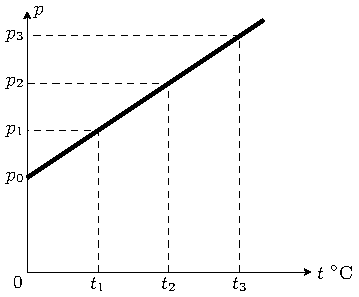
\includegraphics{fig/B/3-10.pdf}
		\caption{气体等容变化的图线}\label{fig_B_3-10}
	\end{minipage}
	\hfill
	\begin{minipage}[t]{0.55\linewidth}
		\centering
		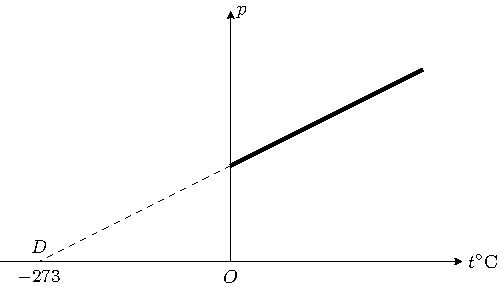
\includegraphics{fig/B/3-11.pdf}
		\caption{}\label{fig_B_3-11}
	\end{minipage}
\end{figure}


查理定律也是在压强不太大、温度不太低的条件下总结出来的.
在这种条件下,不论什么气体都近似地符合这个定律.
当压强很大、温度很低时,每升高1$\Ucede$增加的压强不再等于$p_0$的$1/273$,而且这个数值对不同的气体也不再相同.这时查理定律就不适用了.


\section{热力学温标}\label{sec-B-3-4-thermodynamic-temperature-scale}
图~\ref{fig_B_3-10} 表明了气体的压强跟温度之间的关系.
我们看到,图中的直线并未通过原点,说明气体的压强不是直接与摄氏温度成正比的.但是如果我们改用一个新的温标,那就可以得到压强和温度之间的简单的正比关系.



把图~\ref{fig_B_3-10} 中的直线向左方延长,交横轴于$D$点(图~\ref{fig_B_3-11}),$D$点表示气体的压强等于零时的温度.这个温度是多少度呢?

设$p_t=p_0 \left(1+\frac{t}{273}\right)=0$,由于$p_0\ne 0$,所以必须要求$1+\frac{t}{273}=0$,由此得出$t=-273 \Ucede $.

精确的实验证明,上节查理定律数学表达式中的273应该是273.15.这样,气体压强等于零时的温度就应该是$-273.15 \Ucede $.



英国科学家威廉$\cdot$汤姆孙(开尔文)($1824 \sim 1907$)创立了把$-273.15 \Ucede$作为零度的温标,叫做\NoteBold{热力学温标}(或\NoteBold{绝对温标}),用热力学温标表示的温度叫做\NoteBold{热力学温度}(或\NoteBold{绝对温度}).

热力学温度是国际单位制中七个基本量之一,用符号$T$表示.
它的单位是开尔文,简称为开,国际符号为K.热力学温度的零度是$-273.15 \Ucede$,叫做绝对零度.就每一度的大小来说,热力学温度和摄氏温度是相同的,所以热力学温度跟摄氏温度间的关系为
\[T=t+273.15 \]
为了简化,可以粗略地取$-273 \Ucede $为绝对零度,这样就有
\[T=t+273 \]
例如,在1标准大气压下,冰的熔点为0$\Ucede$即$273 \UK $,水的沸点为100$\Ucede$即$373 \UK$.

利用热力学温标可以使查理定律的表述简化.设在体积不变的情况下,一定质量的气体温度为$t_1$时压强为$p_1$,温度为$t_2$时压强为$p_2$,那么
\[\begin{split}
p_1&=p_0\left(1+\frac{t_1}{273}\right)=p_0\frac{273+t_1}{273}\\
p_2&=p_0\left(1+\frac{t_2}{273}\right)=p_0\frac{273+t_2}{273}\\
\end{split} \]
其中$p_0$表示0$\Ucede$时的压强.把上面两式相除得到
\[\frac{p_1}{p_2}=\frac{273+t_1}{273+t_2} \]
用热力学温度$T_1$和$T_2$分别代换$(273+t_1)$和$(273+t_2)$,得到
\[\frac{p_1}{p_2}=\frac{T_1}{T_2} \]
可见查理定律可以表述为:\NoteBold{体积不变时,一定质量的气体的压强跟热力学温度成正比}.

上面是把查理定律“外推”到零压强而引入热力学温标的.
这种“外推”是可以理解的.随着温度的降低,气体分子热运动减弱,分子对器壁的撞击作用也减弱,因而压强减小.由此推想,在某一个温度下,气体压强变为零,这个温度就是绝对零度.实际上,在达到绝对零度之前,任何气体都已液化甚至变为固体,查理定律早已不适用了.虽然如此,由“外推”得到的绝对零度仍具有物理意义,它是低温的极限,能够无限接近,但不可能达到.

\subsection*{练习三}

\begin{enumerate}
    \item 炎热的夏天,打足了气的自行车胎在日光曝晒下有时会胀破.
    解释这个现象.
\item 乒乓球挤瘪后,放在热水里泡一会,会重新鼓起来.解释这个现象.
\item 一定质量的氢气在0$\Ucede$时的压强是700毫来汞柱,它在30$\Ucede$时的压强是多大?压强为650毫米汞柱时它的温度
是多少摄氏度?保持氢的体积不变.
\item 一定质量的某种气体,在20$\Ucede$时的压强是$1.0\times 10^5$帕.
如果保持它的体积不变,温度升高到50$\Ucede$时,它的压强是多大?温度降低到$-7 \Ucede $时,它的压强又是多大?
\item 盛有氧气的钢筒,在室内(室温是17$\Ucede$)测得筒内气体的压强是$9.31\times 10^6$帕.
当钢筒搬到温度是$-13 \Ucede$的工地时,筒内气体的压强变为$8.15\times 10^6$帕.钢筒是不是漏了气?为什么?
\item 装在容器中的气体,体积为4升,压强为$2.0\times 10^5$帕,温度为300开.
先让气体发生等容变化,压强增大为原来的2倍.
然后让气体发生等温变化,压强又降低到原来的数值.求气体在末状态时的体积和温度.

\end{enumerate}

\section{理想气体的状态方程}
前面我们研究了一定质量的气体在温度不变时压强跟体积的关系以及体积不变时压强跟温度的关系,分别得出了玻意耳--马略特定律和查理定律.现在我们从这两个实验定律出发,确定一定质量的气体的体积、压强、温度这三个状态参量在变化中的相互关系.

设有一定质量的气体,在初状态时的压强、体积和温度分别为$p_1 $,$ V_1 $,$ T_1$,经过某个变化过程,到末状态时这三个量分别变成$p_2 $,$ V_2 $,$ T_2$.气体从初状态到末状态可以经过各种不同的变化过程.
现在设想有一个变化过程是分两个阶段进行的.在第一个阶段中,保持温度$T_1$不变,体积从$V_1$变成$V_2$,压强从$p_1$变成另一个值$p_c$(图~\ref{fig_B_3-12a} 和图~\ref{fig_B_3-12b}).在第二个阶段
中,保持体积$V_2$不变,温度从$T_1$变成$T_2$,压强从$p_c$变成$p_2$(图~\ref{fig_B_3-12b} 和图~\ref{fig_B_3-12c}).

\begin{figure}[htbp]
    \centering
    \begin{subfigure}{0.3\linewidth}
        \centering
        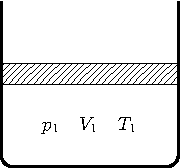
\includegraphics{fig/B/3-12a.pdf}
        \caption{}\label{fig_B_3-12a}
    \end{subfigure}
    \hfil
    \begin{subfigure}{0.3\linewidth}
        \centering
        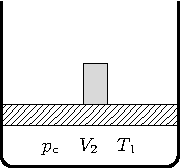
\includegraphics{fig/B/3-12b.pdf}
        \caption{}\label{fig_B_3-12b}
    \end{subfigure}
    \hfil
    \begin{subfigure}{0.3\linewidth}
        \centering
        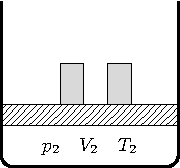
\includegraphics{fig/B/3-12c.pdf}
        \caption{}\label{fig_B_3-12c}
    \end{subfigure}
    \caption{导出气体状态方程的附图.从左到右依次经过等温、等容两个过程.}\label{fig_B_3-12}
\end{figure}

第一个阶段是等温变化,根据玻意耳--马略特定律有
\begin{equation}\label{eq_B_3-1}
p_1V_1=p_cV_2
\end{equation}
第二个阶段是等容变化,根据查理定律有
\begin{equation}\label{eq_B_3-2}
\frac{p_c}{T_1}=\frac{p_2}{T_2}
\end{equation}
由 \eqref{eq_B_3-1} 式解出$p_c$,代入 \eqref{eq_B_3-2} 式,整理后得到
\begin{equation}\label{eq_B_3-3}
\frac{p_1V_1}{T_1}=\frac{p_2V_2}{T_2}
\end{equation}

上式说明,一定质量的气体从初状态$(p_1,V_1,T_1)$变到末状态$(p_2,V_2,T_2)$,压强和体积的乘积与热力学温度的比值是不变的,即
\begin{equation}\label{eq_B_3-4}
\frac{pV}{T}=\text{恒量}
\end{equation}

我们知道,玻意耳--马略特定律和查理定律是在压强不太大、温度不太低的条件下总结出来的.在这种条件下,不论什么气体都近似地符合这两个实验定律.\eqref{eq_B_3-4} 式是从上述两个实验定律推导出来的,因此,也只有在这种条件下,不论什么
气体才近似地符合 \eqref{eq_B_3-4} 式.尽管如此,为了研究的方便,我们还是可以设想出一种气体,能够在任何温度和压强下都遵守 \eqref{eq_B_3-4}  式,这样的气体叫做\NoteBold{理想气体}.\eqref{eq_B_3-4} 式叫做一定质量的理想气体的状态方程.

当然,理想气体是不存在的,它只是实际气体在一定程度上的近似.有许多实际气体,特别是那些不易液化的气体,如氢气、氧气、氮气、空气、氦气等,在通常的温度和压强下,它们的性质很近似于理想气体,可以把它们当作理想气体来处理.这样处理的结果,误差很小,可是计算起来却简便多了.

理想气体状态方程实际上包含了前面讲的两个气体实验
定律.
如果保持温度$T$不变,便得到$pV=\text{恒量}$,这就是玻意耳--马略特定律.如果保持体积$V$不变,便得到$p/T=\text{恒量}$,这就是查理定律.

从理想气体状态方程还可以知道,压强保持不变时,一定质量气体的体积怎样随着温度而变化,这种变化叫做\NoteBold{等压变化}.在保持压强$p$不变时,得到$V/T=\text{恒量}$,这表示\NoteBold{压强不变时,一定质量气体的体积跟热力学温度成正比}.这个关系最初是法国科学家盖$\cdot$吕萨克($1778 \sim 1850$)研究气体热膨胀时得到的实验定律,叫做\NoteBold{盖$\cdot$吕萨克定律}.在压强不太大、温度不太低时,不论什么气体都近似地符合这个定律.


\subsection*{练习四}

\begin{enumerate}
    \item 对一定质量的气体来说,能否做到:
    \begin{enumerate}
    \item    保持压强和温度不变而改变它的体积?
    \item    保持温度和体积不变而改变它的压强?
    \item    保持体积和压强不变而改变它的温度?     
    \end{enumerate}
\item  对一定质量的气体来说,能否做到:
\begin{enumerate}
\item 保持压强不变,同时升高温度并减小体积?
\item 保持温度不变,同时增加体积并减小压强?
\item 保持体积不变,同时增加压强并降低温度?
\end{enumerate}

\item  一定质量的空气,27$\Ucede$时的体积为$1.0\times 10^{-2} \Umc$.计算在压强不变的情况下,温度升高到100$\Ucede$时的体积.
\item  某种柴油机的气缸容积为$0.83\times 10^{-3} \Umc$.压缩前其中空气的温度为47$\Ucede$,压强为$0.8\times 10^5$帕.
在压缩冲程,活塞把空气压缩到原体积的1/17,压强增大到$40\times 10^5$帕.求这时空气的温度.
\item  在容积为25升的容器中,盛有温度为37$\Ucede$、压强为62标准大气压的氧气.求氧气在标准状态($0 \Ucede$,1标准大气压)下的体积.
从化学课中学过,在标准状态下,1摩的任何气体的体积都是22.4升.你能不能由此求得容器中氧气的摩尔数并进而求得氧气的质量?怎样求?
\item  一个瓶子里装有某种气体,瓶上有一个小孔跟外面大气相通.原来瓶里气体的温度为15$\Ucede$.如果把它加热到207$\Ucede$,瓶里保留的气体的质量是原来质量的几分之几?
\item  贮气筒内装有压缩气体,温度是27$\Ucede$,压强是$40\times 10^5$帕.
如果从筒内放出一半质量的气体,并使筒内剩余的气体的温度降到12$\Ucede$,这些剩余气体的压强是多大?

\end{enumerate}


\section{克拉珀龙方程}
\subsection{摩尔气体恒量} 

上一节讲的气体状态方程
\[\frac{pV}{T}=\text{恒量} \]
是一定质量的理想气体状态方程,其中的恒量跟气体的质量有关系.在体积和温度相同的情况下,气体的质量越多,气体的压强就越大,因而上式中的恒量就越大.自行车车胎里打进的空气越多,车胎胀得越硬,这是大家都知道的.

实验表明,上式中的恒量还跟气体的种类有关系.在体积和温度相同的情况下,质量相同的不同种类气体,它们的压强并不相同,因而上式中的恒量也不相同.

那么,怎样在一般情况下应用上式呢?我们先把上式用于质量限定的各种气体,而且质量就限定为1摩尔.这是因为,在标准状态下,即$p_0=1$标准大气压,$T_0=273 \UK $,1摩的任何气体的体积都是$V_0=22.4$升.由此我们可以求得一个适用于1摩尔任何气体的恒量,叫做\NoteBold{摩尔气体恒量}.
它通常用$R$来表示,即
\[R=\frac{p_0V_0}{T_0} \]

$R$的数值跟$p $,$ V $,$ T$的单位有关.在国际单位制中,$p_0=
1.013\times 10^5 \UPa=1.013\times 10^5 \UNmq$,$V_0=22. 4\times 10^{-3} \Umcmol$,$T_0=273 \UK $,代入上式得到
\[\begin{split}
R&=\frac{1.013\times 10^5 \UNmq \times  22. 4\times 10^{-3} \Umcmol}{273\UK }\\
&=8.31 \UJmolK 
\end{split} \]

对于1摩的理想气体,因为$pV/T=p_0V_0/T_0=R$,所以
$$pV=RT$$
这就是1摩的理想气体的状态方程,它对任何气体都适用.

摩尔气体恒量是热学中又一个重要常数.
不仅在研究气
体的热学性质中,而且在研究其他热现象中,它与阿伏伽德罗常数共同起着重要作用.

\subsection{克拉珀龙方程} 

知道了1摩的理想气体的状态方程,我们不难得到任意质量的理想气体的状态方程.设有质量为$m$千克的某种理想气体,它的摩尔质量为$M \Ukgmol $,它的摩尔数$n=m/M$摩.既然1摩的理想气体在标准状态下占有体积$V_0$($=22.4 \UL $),那么$n$摩的理想气体在标准状态下占有的体积应为$V'_0=nV_0$.由理想气体的状态方程可得:
\[\begin{split}
\frac{pV}{T}&=\frac{p_0V'_0}{T_0}\\
&=n\frac{p_0V_0}{T_0}=nR
\end{split} \]
由此得到
\[pV=nRT \]
或\[pV=\frac{m}{M}RT \]
这就是任意质量的理想气体的状态方程,又叫做\NoteBold{克拉珀龙方程}.只要温度不太低,压强不太大,这个方程对一切气体都适用.
这个方程在实际中有广泛的应用,可以用来解决有关气体的各种问题.

\begin{example}
容积为30升的瓶内装有氢气.假定在气焊过程中,温度保持27$\Ucede$不变,当瓶内压强由$4. 9\times 10^6$帕降为$9.8\times 10^5$帕时,共用去多少氢气?
\end{example}

\begin{solution}
用国际单位制来计算,把已知各个量的数值用相应的单位表示出来.
$p_1=4.9\times 10^6 \UPa $;$V=30\UL=30\times 10^{-3}\Umc$;$p_2=9.8\times 10^5\UPa$;$T=(27+273)\UK=300\UK$;$M=2\times 10^{-3} \Ukgmol$.

这个例题可以这样来解:根据克拉珀龙方程先计算瓶内原有氢气的质量$m_1$,再计算气体状态改变后瓶内氢气的质量$m_2$,二者之差$m_1-m_2$就是用去的氢气的质量.

气体的初状态和末状态的体积$V$和温度$T$保持不变,压强$p$和质量$m$发生了变化,压强由$p_1$变到$p_2$,质量由$m_1$变到$m_2$.

由
\[
p_1V=\dfrac{m_1}{M}RT
\]
得到
\[
m_1=\dfrac{p_1VM}{RT}
\]
由
\[
p_2V=\dfrac{m_2}{M}RT
\]
得到
\[
m_2=\dfrac{p_2VM}{RT}
\]
所以
\[m_1-m_2=\frac{VM}{RT}(p_1-p_2) \]
代入数值得到
\[\begin{split}
m_1-m_2&=\frac{30\times 10^{-3}\times 2\times 10^{-3}}{8.31\times 300}(4.9\times 10^6-9.8\times 10^5)\Ukg\\
    &=9.4\times 10^{-2} \Ukg
\end{split} \]
\end{solution}

如果就一定质量的气体来考虑气体的状态变化,即压强由$p_1$降低到$p_2$,而体积由$V_1$膨胀到$V_2$,能不能解出这个题目?你来试一下,并把两种解法加以比较.

利用理想气体状态方程解题,首先要明确我们所研究的对象是哪部分气体,以及气体状态发生变化时它的初状态和末状态,然后才能用状态方程来求解.
计算时要注意物理量的单位.
$T$必须采用热力学温度,根据$p_1V_1/T_1=p_2V_2/T_2$解题时,公式两边的$p$和$V$的单位必须统一.
根据$pV=mRT/M$解题时,$R$的单位必须与$p$、$V$的单位相适应.

\subsection*{练习五}

\begin{enumerate}
    \item 如果压强用标准大气压作单位,体积用升作单位,试通过计算证明:$R=0.082 \UatmLmolK $.
\item 一个容器内装有氧气100克,压强为10标准大气压,温度为47$\Ucede$,容器的容积是多少$\UmcA$?
\item 1克的气体,温度为27$\Ucede$、压强为600毫米汞柱时,体积为5升.
2克的同种气体,温度为127$\Ucede$、压强为400毫米汞柱时,体积是多少升?
\item 容积是10升的钢筒里盛有90标准大气压、$-13 \Ucede $的氧气,求钢筒中氧气的质量.已知氧气在标准状态下的密度$\rho_0=1.43 \Ukgmc$.
\item 有0.612克的某种氮氧化合物,在293开和1标准大气压时体积为480$\Ucmc$.
这是一种什么气体?写出它的分子式.
\item 给汽车轮胎打气,使胎内空气达到所需的压强,冬天和夏天打入胎内的空气质量是否相同?冬天还是夏天打入的空气质量多?
\item 有两种不同种类的气体,它们的温度和体积都相同.如果它们的质量也相同,气体的压强是否相同?如果它们的质
量不同,但摩尔数相同,气体的压强是否相同?
\item 理想气体的状态方程可写成$pV/T=C(\text{恒量})$.
对于这个恒量$C$,下面哪种说法正确,哪种说法错误,并说明理由.
\begin{enumerate}
\item 对质量相同的任何气体,$C$都相同.
\item 对质量不同的同种气体,$C$都相同.    
\item 对摩尔数不同的同种气体,$C$都相同.
\item 对摩尔数相同的任何气体,$C$都相同.
\end{enumerate}
\end{enumerate}

\section{气体分子运动的特点}\label{sec-B-3-7-characteristics-of-gas-molecular-motion}
\subsection{分子间的距离较大} 
气体很容易被压缩,说明气体分子间的距离比较大.
气体凝结成液体时,体积要缩小上千倍,而液体不容易被压缩,可以认为其中的分子几乎是紧密排列的,可见气体分子之间的距离大约是分子直径的$\sqrt[3]{1000}$倍,即10倍.由于气体分子间的距离比较大,所以在处理某些问题时可以把气体分子看作是没有大小的质点.也是由于气体分子间的距离比较大,分子间的相互作用力十分微弱,所以通常可以认为,气体分子除了相互碰撞或者跟器壁碰撞外不受力的作用,可以在空间里自由移动.由此可以说明:气体能充满它所能达到的空间,既没有一定的体积,没有一定的形状.

\subsection{分子间的碰撞频繁} 
比起固体和液体来,气体中的分子是比较稀疏的.
但是单位体积中的分子数还相当大.在标准状态下,1$\Ucmc$气体中仍含有$2.7\times 10^{19}$个分子.
大量分子永不停息地运动,分子之间不断地发生碰撞.
在标准状态下,一个空气分子在1秒内与其他空气分子的碰撞竟达65亿次之多.频繁的碰撞使得每个分子的速度的大小和方向频繁地改 
变.设想我们追随某个气体分子的运动(图~\ref{fig_B_3-13}),我们将看到这个分子的运动是忽左忽右,忽前忽后,时快时慢,运动轨迹是一条极不规则的折线.
频繁的碰撞造成气体分子做杂乱无章的热运动.
\begin{figure}[htbp]
    \centering
    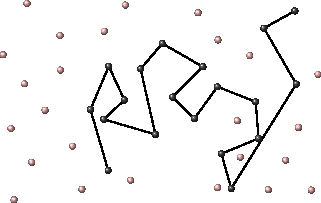
\includegraphics{fig/B/3-13.pdf}
    \caption{气体分子间的碰撞}\label{fig_B_3-13}
\end{figure}

通常假定分子之间或分子与器壁之间的碰撞是完全弹性碰撞.

\subsection{分子沿各方向运动的机会均等} 

气体分子做杂乱无章的热运动,就某一个分子来说,它在某一时刻的速度具有怎样的大小和方向,完全是偶然的.但是,对大量分子的整体来说,分子的运动却表现出一定的规律.
先来讨论分子运动的方向.正因为大量分子的运动十分混乱,在某一时刻向任一方向运动的分子都有,因而可以想见,在任一时刻分子沿各方向运动的机会是均等的,没有任何一个方向,沿着它运动的分子的数目更多.
设想真有这么一个方向,那么,由于气体分子的频繁碰撞,分子的运动越来越混乱,这个方向也不会存在了.
这就是说,气体分子沿各个方向运动的数目应该是相等的.

这里所说的数目相等,是对大量分子用统计方法得到的一个统计平均数,与实际数目会有微小的出入.
分子数越多,这种用统计方法得到的结果跟实际情况越符合.
用分子运动论的观点研究热现象,涉及的总是大量分子,统计方法非常有用.

\subsection{分子速率按一定规律分布} 
大量分子做无规则运动,速率有的大,有的小,但分子的速率却按照一定的规律分布.

研究表明,气体的大多数分子,速率都在某个数值附近,离开这个数值越远,分子数越少,表现出“中间多,两头少”的
分布规律.
表 \ref{tab_B_3-1} 是氧气分子速率的分布情况.我们看到,在0$\Ucede$时速率在$300\sim 400\Ums$这一速率区间的分子数最多,速率大于400$\Ums$和小于300$\Ums$的分子数依次递减,速率很大和很小的分子实际上很少.
温度升高时,这种“中间多,两头少”的分布规律虽然不变,可是与分子数的最大值相对应的速率区间却移向速率大的一方,也就是说,温度升高时,速率小的分子数减少,速率大的分子数增加.
这种速率分布规律是一种统计规律.
表中的在某一速率区间的相对分子数,也是
对大量分子用统计方法得到的统计平均数,与实际数值会有微小的出入.

\begin{table}[htbp]
    \centering
    \caption{氧气分子的速率分布}\label{tab_B_3-1}
    \begin{tblr}{ccc}
		\toprule
		\SetCell[r=2]{c} {按速率大小划分的区间\\($\Ums$)}
		 & \SetCell[c=2]{c} {各速率区间的分子数占\\总分子数的百分率($\%$)}&\\
		& $0 \Ucede $ & $100 \Ucede$ \\
		\midrule
		100以下 & 1.4 & 0.7\\
		$100\sim 200$ &    8.1 &    5.4
		\\
		$200\sim 300$ &    7.0     &11.9
		\\
		$300\sim 400$ &    21.4 &    17.4
		\\
		$400\sim 500$ &    20.4 &    18.6
		\\
		$500\sim 600$ &    15.1 &    16.7
		\\
		$600\sim 700$ &    9.2 &    12.9
		\\
		$700\sim 800$  &    4.5 &    7.9
		\\
		$800\sim 900$ &    2.0 &    4.6
		\\
		900 以上 &    0.9 &    3.9\\
		\bottomrule
    \end{tblr}
\end{table}

既然在一定温度下,某种气体的分子速率分布是确定的,我们就可以求出在这个温度下该种气体分子的平均速率,即所有分子的速率的平均值.温度升高时,速率大的分子数增
加,分子的平均速率增大.例如氮气分子的平均速率在$-150 \Ucede $时为320$\Ums$,在$0\Ucede$时为493$\Ums$,在$1000 \Ucede $时
为1194$\Ums$.这里我们又一次看到,温度越高,分子的热运动越激烈.

\section{气体实验定律的微观解释}
\subsection{气体压强的微观解释} 
从气体分子运动论的观点看来,气体压强是大量的气体分子频繁地碰撞器壁而产生的.雨滴打在雨伞上,使伞面受到冲力,单个雨滴对伞面的冲力是短暂的,但大量密集的雨滴接连不断地打在伞面上,对伞面就形成一个持续的均匀的压力.
同样,单个分子碰撞器壁的冲力是短暂的,但是大量分子频繁地碰撞器壁,就对器壁产生持续的均匀的压力.
下面我们从气体分子运动论的观点定性地讨论一下气体的压强.

设想容器内只有一个分子,我们可以利用以前学过的力学知识算出这个分子碰撞器壁时对器壁产生多大的冲力.
现在的问题是:容器中有大量分子,它们的速度的大小和方向又不断地在改变.怎样才能算出大量分子碰撞器壁时对器壁产生的冲力呢?

我们知道,气体分子做无规则运动,它们沿各个方向运动的机会是均等的,也就是说,在上下、前后、左右各个方向中没有哪个方向的运动占优势.
因此我们可以认为各有1/6的分子向着上下前后左右这六个方向运动.
气体分子速度的大小也不相同,但我们可以认为所有分子都以平均速率向着各个
方向运动.



现在设想有一个向右运动的分子与器壁发生碰撞(图~\ref{fig_B_3-14}).
碰撞前的动量是$mv$,其中$v$是分子的平均速率,碰撞后向左运动,速率是$v'$,动量是$-mv'$.这个分子碰撞前后的动量变化是$-mv'-mv$.气体分子与器壁之间的碰撞是完全弹性碰撞,这样,分子碰撞前后的速率相等,即$v'=v$,因而动量变化是$-2mv$.从动量定理知道,这个动量变化$-2mv$等于器壁对分子的冲量.从牛顿第三定律知道,这时分子对器壁也有一个大小相等方向相反的冲量.可见气体分子每碰撞一次器壁,就给器壁$2mv$的冲量.

\begin{figure}[htbp]
	\centering
	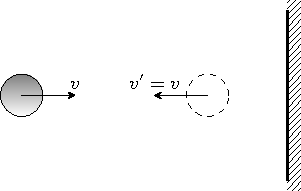
\includegraphics{fig/B/3-14.pdf}
	\caption{气体分子每碰撞一次器壁,就给器壁$2mv$的冲量.}\label{fig_B_3-14}
\end{figure}



在一段时间内,大量分子与器壁碰撞多少次,分子给器壁
的总冲量就是$2mv$的多少倍.
而在单位时间内分子给器壁的总冲量就等于器壁所受的压力,单位面积器壁所受的压力就等于气体的压强.

这样,如果知道单位时间内分子对单位面积器壁的碰撞次数,就可以求得气体的压强.这个碰撞次数跟单位体积内气体的分子数有关.
单位体积内气体的分子数越多,即气体分子越密,这个碰撞次数就越多.
这是容易理解的.
这个碰撞次数还跟分子的平均速率有关.如图~\ref{fig_B_3-15} 所示,我们在气体内部设想一个柱体,底面积为单位面积,高为平均速率的数值.在单位时间内,这个柱体中向右运动的分子都会运动到器壁而发生碰撞.平均速率越大,这个柱体越高,其中的分子越多,分子与器壁发生碰撞的次数就越多.可见,单位时间内分子对单位面积器壁的碰撞次数是由单位体积内的分子数和分子的平均速率决定的.由此我们将不难理解气体压强也是由单位体积内的分子数和分子的平均速率决定的.
单位体积内的分子数越多,分子的平均速率越大,气体的压强就越大.
\begin{figure}[htbp]
    \centering
    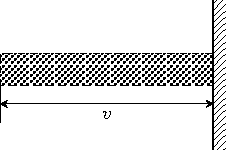
\includegraphics{fig/B/3-15.pdf}
    \caption{单位时间内分子对单位面积器壁的碰撞次数跟分子的平均速率有关.}\label{fig_B_3-15}
\end{figure}

\subsection{气体实验定律的微观解释} 
知道了气体压强是由什么决定的,我们就能够用气体分子运动论对气体实验定律作出微观解释.

一定质量的气体,温度保持不变,也就是分子的总数和分
子的平均速率保持不变.在这种情况下,气体的体积减小到原来体积的几分之一,单位体积内的分子数就增大到原来的几倍,气体的压强就增大到几倍.
气体体积增大时,情况恰好相反.
结果是气体的压强与体积成反比.
这就是玻意耳--马略特定律.

用气体分子运动论也可以解释查理定律.
一定质量的气体,体积保持不变而温度升高时,分子的平均速率增大,因而气体的压强增大.
温度降低时,情况恰好相反.

怎样解释盖$\cdot$吕萨克定律呢?从气体分子运动论可以说明:一定质量的气体温度升高时,要保持压强不变,只有让气体的体积增大才行.这时,一方面由于温度升高,分子的平均速率增大,以致每次碰撞给器壁的冲量增加,同时单位时
间内对单位面积器壁的碰撞次数增多,使压强有增大的倾向;另一方面,由于体积增大,单位体积内的分子数减少,以致单位时间内分子对单位面积器壁的碰撞次数减少,使压强有减小的倾向.
当体积增大到一定程度时,这两种倾向抵消,所以压强保持不变.

气体分子运动论不仅能够解释上述气体实验定律,而且能够解释气体的其他一些性质,如气体的比热、扩散、热传导等.
气体分子运动论是热学和分子物理学的重要组成部分,它使人们对气体的研究从宏观领域进入微观领域,扩展和加深了人们对气体性质的认识.


\subsection*{练习六}

\begin{enumerate}
    \item 现在我们用另一种方法估算一下气体分子间的距离与分子直径的关系.在标准状态下,1摩的气体占有22.4升的体积.我们设想其中的每个分子都位于一个小立方体的中心.这个小立方体的边长是多少?分子直径的数量级为$10^{-10}$米.把小立方体的边长跟分子直径相比较,结果怎样?
\item 根据第\ref{sec-B-3-7-characteristics-of-gas-molecular-motion}节表 \ref{tab_B_3-1} 中的数据能不能估算出0$\Ucede$和100$\Ucede$时氧气分子的平均速率?怎样估算?结果怎样?
\end{enumerate}

\section{理想气体的内能}
从气体分子运动论的观点看来,所谓理想气体,是指分子间没有相互作用和分子可以看成没有大小的质点的气体.这就是理想气体的微观模型.
一定质量的气体,温度越高,压强
越小,因而气体越稀薄,气体分子间的距离越大,就越接近于理想气体.在温度较低和压强较大的情况下,气体不那么稀薄,在研究气体的性质时必须考虑到分子的大小和分子间的相互作用,而它们跟气体的种类有关,这时气体不再遵守理想气体状态方程,并且显示出不同气体在性质上的差异.

理想气体的分子之间既然没有相互作用,就不存在分子势能.
因此,理想气体的内能就是气体所有分子热运动的动能的总和.
分子的动能跟气体的温度有关,分子势能跟气体的体积有关.
现在不存在分子势能,因而理想气体的内能只跟温度有关,跟体积无关.这就是说,只要温度保持不变,气体的体积增大一些因而气体分子疏一些,或者气体的体积减小一些因而气体分子密一些,不仅分子动能保持不变,分子势能仍旧不存在,因此理想气体的内能保持不变.

\section{理想气体的内能变化$^\star$}
前面我们讲过了理想气体的等温、等容和等压变化,现在我们分析一下在这三种等值变化中内能的变化.

设一定质量的理想气体在温度不变的情况下发生膨胀,由初状态变到末状态.
由于温度保持不变,所以气体的内能也不变,即$\Delta E=0$.气体发生膨胀时对外做功,所以$W$为负值,即$W<0$.从热力学第一定律$W+Q=\Delta E=0$知道,$Q$应为正值,即$Q>0$,而且$W$和$Q$的绝对值相等.可见,在等温膨胀的过程中,理想气体要从外界吸收热量,吸收的热量并没有增加气体的内能,而全部用来对外做功.

在体积不变的情况下,对一定质量的理想气体加热,使它的温度升高,压强增大,由初状态变到末状态.末状态的温度比初状态高,所以内能增加,即$\Delta E>0$.气体的体积不变,外界既没有对气体做功,气体也没有对外界做功,所以$W=0$.根据热力学第一定律我们得到$Q=\Delta E$.可见,在等容变化中,如果理想气体从外界吸收热量,这个热量就全部用来增加气体的内能.

在压强不变的情况下,对一定质量的理想气体加热,使它的温度升高,体积增大,由初状态变到末状态.
末状态的温度比初状态高,所以内能增加,即$\Delta E>0$.
气体膨胀对外做功,$W<0$.从热力学第一定律$W+Q=\Delta E>0$知道,这时气体吸收的热量$Q$的绝对值大于$W$的绝对值.
这就是说,在等压膨胀的过程中,理想气体从外界吸收的热量,一部分用来增加气体的内能,一部分用来对外做功.

除了上述三种等值变化外,还有一种所谓绝热变化在实际中常常遇到.
物体在状态的变化过程中如果跟外界没有热交换,这种变化就叫做\NoteBold{绝热变化}.
绝热变化的特点是:$Q=0$.用绝热良好的材料把容器包起来,让气体发生膨胀或者对气体进行压缩,这时的变化就可以看作绝热变化.
气体的膨胀或压缩进行得很迅速,从初状态到末状态所用的时间很短,气体来不及跟外界发生热交换,这种迅速的变化也可以看作绝热变化.
图~\ref{fig_B_2-1} 所示的压缩气体的演示,热机气缸内气体膨胀做功,过程进行得很迅速,都可以看作绝热变化.在绝热压缩的过程中,外界对气体所做的功完全用来增加气体的内能,使气体的温度升高.在绝热膨胀的过程中,气体对外界做功
完全靠气体内能的减少,因而气体的温度降低.


\subsection*{练习七}
\begin{enumerate}
    \item 一定质量的理想气体在温度不变的情况下被压缩,气体的内能是否改变?外界对气体是否做功?气体从外界吸热还是向外界放热?功和热量有什么关系?
\item 一定质量的理想气体在体积不变的情况下压强减小,这时外界对气体是否做功?气体的内能是否改变,怎样改变?气体放出的热量跟内能的改变有什么关系?
\item 一定质量的理想气体在压强不变的情况下体积减小,外界对气体是否做功?气体的内能是否改变,怎样改变?气体放热还是吸热?这个热量跟内能的改变有什么关系?
\end{enumerate}



\section*{复习题}

\begin{enumerate}
	\item 
	哪几个物理量是描述气体的状态参量?
	
	\item \label{review_B_3-2}
	什么叫等温变化?玻意耳--马略特定律的内容是什
	么?写出它的表达式.
	
	\item \label{review_B_3-3}
	什么叫等容变化?查理定律的内容是什么?写出它的
	表达式.
	
	\item \label{review_B_3-4}
	什么叫等压变化?盖$\cdot$吕萨克定律的内容是什么?写
	出它的表达式.
	
	\item 
	写出任意质量的理想气体的状态方程即克拉珀龙方
	程,并作为特例推出:1摩的理想气体的状态方程,质量一定
	但不知道质量数值时理想气体的状态方程,(\ref{review_B_3-2})、(\ref{review_B_3-3})、(\ref{review_B_3-4})中的
	三个气体实验定律.
	
	
	
	\item 
	你自己总结一下用理想气体状态方程解题的基本思
	路和步骤以及要注意的问题.
	
	\item 
	气体分子运动的特点是什么?从分子运动论的观点
	看来,气体压强是怎样产生的?它的大小是由什么决定的?
	
	\item 
	用气体分子运动论对三个气体实验定律作出微观解
	释.
	
	\item 
	理想气体的微观模型是怎样的?为什么理想气体的
	内能只跟温度有关,而跟体积无关?
	
	\item$^\star$ 
	试分别说明理想气体在等温、等容、等压变化中内
	能变化的情形.
	
\end{enumerate}


\section*{习题}
\begin{enumerate}
    \item 下面几种说法,哪个正确,哪个错误,并说明理由.
    \begin{enumerate}
        \item 有两个相同的容器,内装同种气体,它们的压强相同,因而它们的温度一定相同.
        \item 有两个相同的容器,内装质量相同的不同气体,它们的压强不同,因而它们的温度一定不同.
        \item 有两个相同的容器,内装摩尔数相同的气体,它们的压强相同,因而它们的温度一定相同.
    \end{enumerate}
\item 一定质量的理想气体,处在某一初始状态.
现在要使气体的温度经过状态变化后回到初始状态的温度,用下列哪些过程可能实现?
\begin{enumerate}
    \item 先保持压强不变而使它的体积膨胀,接着保持体积不变而减小压强.
\item 先保持压强不变而使它的体积减小,接着保持体积不变而减小压强.
\item 先保持体积不变而增大压强,接着保持压强不变而使它的体积膨胀.
\item 先保持体积不变而减小压强,接着保持压强不变而使它的体积膨胀.     
\end{enumerate}
\item 盖$\cdot$吕萨克定律如果用摄氏温标$t$来表示,可以写成下式:
\[V_t=V_0\left(1+\frac{t}{273}\right) \]
其中$V_0$和$V_t$分别表示气体在$0 \Ucede$和$t \Ucede$时的体积.试推导出上式.
\item 能不能根据玻意耳--马略特定律和盖$\cdot$吕萨克定律推出一定质量的理想气体的状态方程$PV/T=$恒量?实际推导一下.
\item 当温度为27$\Ucede$、压强为$2.0\times 10^5$帕时,32克氧气的体积是多大?密度是多大?另有48克氧气,温度和压强跟上述数值相同,氧气的密度又是多大?    
\item   试根据克拉珀龙方程推导出用压强和温度来表示的气体密度的表达式.
\item  水银气压计中混入了一个空气泡,上升到水银柱的上方,使水银柱上方不再是真空,因而气压计的读数比实际的大气压小些.
当实际大气压为768毫米汞柱时,气压计的读数只有750毫米汞柱,此时管中水银面到管顶的距离为80毫米.
当气压计读数为740毫米汞柱时,实际大气压为多少?设温度保持不变.
\item  在湖面下50米深处(温度为$4 \Ucede$)有一个体积为$10 \Ucmc$的气泡升到湖面上来,湖面的温度为17$\Ucede$,求它升到湖面时的体积.
大气压强为$1.013\times 10^5$帕.
\item  有两个容积相等的容器,里面盛有同种气体,用一段水平玻璃管把它们连结起来.在玻璃管的正中央有一段水银柱,当一个容器中气体的温度是0$\Ucede$,另一个容器中气体的温度是20$\Ucede$时,水银柱保持静止.
如果使两容器中气体的温度都升高10$\Ucede$,管中的水银柱会不会移动?如果移动的话,向哪个方向移动?试根据学过的气体定律加以说明.
\item  一个容器,如果其中气体十分稀薄,通常就说这个容器为“真空”.有一个容积为10$\Ucmc$的电子管,在温度为300开时用真空泵把它抽成真空,使管内气体压强为 $5\times 10^{-6}$毫米汞柱,这时管内有多少个气体分子?
\item  氧气瓶的容积是32升,其中氧气的压强是130标准大气压.规定瓶内氧气压强降到10标准大气压时就要重新充氧.有一个车间,每天需用1标准大气压的氧气400升.这瓶氧气能用几天?假定温度保持不变.



\item  如图~\ref{fig_B_3-16} 所示,气缸$A$和容器$B$由一细管经阀门
$K$相联.$A$和$B$的壁都是透热的.$A$放在27$\Ucede$、1标准大气压的大气中,$B$浸在127$\Ucede$的恒温槽内.开始时$K$是关断的,
$B$内没有气体,容积$V_B=2.4 \UL $;$A$内装有气体,体积$V_A=
4.8 \UL $.打开$K$,使气体由$A$流入$B$,等到活塞$D$停止移动
时,$A$内气体的体积是多大?假设活塞$D$与气缸壁之间没有摩擦,细管的容积忽略不计.
\begin{figure}[htbp]
	\centering
	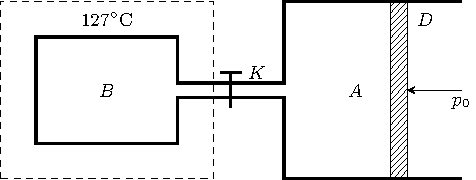
\includegraphics{fig/B/3-16.pdf}
	\caption{}\label{fig_B_3-16}
\end{figure}

\end{enumerate}





